\chapter{Marco Referencial} \label{ch:marcoref}

%\begin{flushright}
%\small\textit{Tanto si piensas que puedes, como si piensas que no puedes, est\'as en lo cierto.}\\
%		\small\textbf{Henry Ford}
%\end{flushright}

%*************************************************************************************************************************************%
	\section{Metodolog\'ia de dise\~{n}o} \label{sec:metodologia}
Este trabajo sigue la metodolog\'ia de dise\~{n}o para sistemas mecatr\'onicos propuesta en \cite{diegoflores_2018} y que tiene como t\'itulo \textit{Design methodology for mechatronic systems: A functional approach}. Esta metodolog\'ia aborda al problema de dise\~{n}o desde un enfoque funcional. Tambi\'en acude a m\'ultiples disciplinas, herramientas y m\'etodos para proponer una soluci\'on m\'as completa y sin\'ergica.\\

\noindent La metodolog\'ia de dise\~{n}o se compone de dos grandes dominios:

\begin{itemize}
	\item Dominio de dise\~{n}o de proyecto.
	\item Dominio de dise\~{n}o.
\end{itemize}

		\subsection*{Dominio de dise\~{n}o de proyecto}
\noindent Es en este dominio se abordan las estrategias y planes del proyecto. Se definen los alcances, las metas, y el ciclo de vida del proyecto. Este dominio se compone de diferentes fases:

\begin{itemize}
	\item Fase de inicializaci\'on. 
	\item Fase de planeaci\'on.
	\item Fase de ejecuci\'on.
	\item Fase de t\'ermino.
\end{itemize}

		\subsection*{Dominio de dise\~{n}o}
\noindent Este dominio es iterativo e incremental. Cada concurrencia en el dise\~{n}o conlleva a un mejor entendimiento del problema, as\'i como a mejores propuestas de soluci\'on. Este dominio est\'a compuesto por las siguientes etapas:

\begin{itemize}
	\item \textbf{Definici\'on del sistema}: en esta etapa se identifican las necesidades que el proyecto deber\'a satisfacer, se definen los requerimientos y se establecen los objetivos. Tambi\'en, se definen los modos de operaci\'on del sistema mecatr\'onico y se tratan de identificar la mayor cantidad de problemas a resolver.
	\item \textbf{Desarrollo del sistema f\'isico}: etapa en la que se lleva a cabo el dise\~{n}o del sistema f\'isico con base en la descripci\'on de la etapa anterior. La etapa de desarrollo del sistema f\'isico est\'a compuesta por los siguientes puntos:
		\begin{itemize}
			\item Desarrollo de las arquitecturas del sistema.
			\item Definici\'on de la estrategia de dise\~{n}o.
			\item Desarrollo del dise\~{n}o preliminar.
			\item Detallado del sistema f\'isico.
\end{itemize}
		
La realizaci\'on de las arquitecturas del sistema incluye a la arquitectura funcional y a la arquitectura f\'isica.
	\item \textbf{Desarrollo del comportamiento del sistema}: en esta etapa se busca maximizar la funcionalidad y el comportamiento del sistema. Esta etapa est\'a compuesta por los siguientes puntos:
		\begin{itemize}
			\item Definici\'on de la estrategia del comportamiento.
			\item Desarrollo del comportamiento del sistema.
			\item Detallado del sistema mecatr\'onico.
		\end{itemize}
Cada comportamiento propuesto debe ser evaluado y seleccionado para mejorar el desempe\~{n}o del sistema.		
	\item \textbf{Modelado y simulaci\'on}: esta etapa se ejecuta de manera paralela a partir del desarrollo del sistema f\'isico y en ella se realizan los modelos y las simulaciones del sistema mecatr\'onico que se est\'a dise\~{n}ando.
	\item \textbf{Validaci\'on y verificaci\'on}: esta etapa se ejecuta en paralelo a partir de la definici\'on del sistema. El prop\'osito de esta etapa es corroborar que se est\'a dise\~{n}ando el sistema correcto y que \'este ejecutar\'a todas sus funciones.
\end{itemize}

\noindent El dominio de dise\~{n}o se encuentra divido en dos subdominios: dominio l\'ogico y dominio f\'isico.
\begin{itemize}
	\item \textbf{Dominio l\'ogico}: en este dominio se lleva a cabo la descomposici\'on de funciones del sistema. Se debe establecer la funci\'on principal del sistema y las subfunciones que de ella derivan. Las funciones deben atender a los requerimientos, nacidos a su vez de las necesidades. 
	\item \textbf{Dominio f\'isico}: en el dominio f\'isico, las funciones son agrupadas en sistemas y subsistemas. Dentro de este domino se establecen las soluciones a cada sistema y subsistema, los cuales deben atender a las funciones planteadas.
\end{itemize}

%*************************************************************************************************************************************%	
	\section{Herramientas de dise\~{n}o} \label{sec:tools}
		\subsection{Descomposici\'on de funciones} \label{subsec:fbs}
La descomposici\'on de funciones (\textit{Functional Breakdown Structure}, FBS) es un desglose estructurado y modular de cada una de las funciones que debe cumplirse para realizar una misi\'on gen\'erica \cite{fbsnasa_2009}. La descomposici\'on de funciones no detalla productos, sino operaciones o actividades que deben realizarse.\\

\noindent La descomposici\'on de funciones no est\'a ligada a ninguna implementaci\'on f\'isica particular debido a que se trata de una lista de las funciones necesarias para cumplir los objetivo de dise\~{n}o y no de elementos o componentes de la implementaci\'on f\'isica.\\

\noindent Realizar esta descomposici\'on de funciones otorga a los dise\~{n}adores total visibilidad de lo que el sistema deber\'a realizar: sirve como una lista de verificaci\'on para asegurar que ninguna funci\'on fue omitida durante el dise\~{n}o, especialmente en las etapas tempranas de la concepci\'on f\'isica del sistema.\\

\noindent La descomposici\'on FBS sirve de gu\'ia en el desarrollo de la implementaci\'on f\'isica del sistema, otorga visibilidad de aquellas tecnolog\'ias que necesitan ser desarrolladas m\'as profundamente para cumplir con las funciones requeridas y ayuda a identificar las habilidades que deber\'a tener el personal que opere el sistema. De igual manera, permite que cada una de las disciplinas de la ingenier\'ia que se encuentran presentes en el desarrollo del sistema se integren en el m\'aximo grado posible. 

		\subsection{Definici\'on de integraci\'on para modelado de funciones} \label{subsec:idef0}
El est\'andar IDEF0 (\textit{Integration Definition for Function Modeling}, IDEF) es un m\'etodo dise\~{n}ado para modelar decisiones, acciones y actividades dentro de la organizaci\'on de un sistema \cite{IDEF0}. El est\'andar IDEF0 posee un lenguaje gr\'afico que asocia el flujo de energ\'ia, materia e informaci\'on entre las diferentes funciones que desempe\~{n}a un sistema.\\

\noindent El objetivo del est\'andar IDEF0 es hacer que el personal pueda entender el comportamiento del sistema desde un punto de vista funcional, tomando en cuenta los diferentes niveles de abstracci\'on.\\

\noindent El bloque constructivo de un diagrama IDEF0 es mostrado en la imagen \ref{img:bloqueidef0}.

\begin{figure}[H]
	\centering
		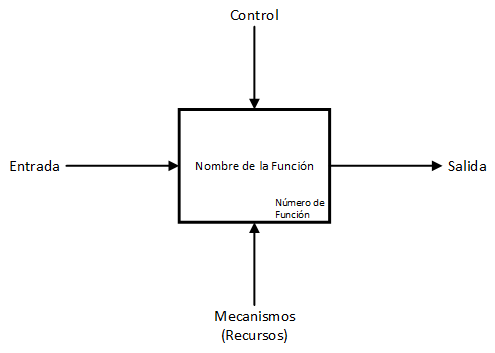
\includegraphics[scale=0.65]{marcoref/IDEFBlock}
	\caption{Bloque constructivo de un diagrama IDEF0.}
	\label{img:bloqueidef0}
\end{figure}

\noindent El bloque mostrado en la imagen \ref{img:bloqueidef0} tiene tres entradas y una salida. Estas entradas y salidas representan lo siguiente:

\begin{itemize}
	\item La se\~{n}al de entrada representa el recurso que ser\'a transformado en algo.
	\item La se\~{n}al de control representa todas aquellas variables o condiciones que dictan que la funci\'on deba realizarse.
	\item La se\~{n}al de mecanismos representa todas aquellas herramientas, t\'ecnicas, procesos, etc., que ayudan o son necesarios para la creaci\'on de la salida o transformaci\'on de la entrada.
	\item La se\~{n}al de salida representa el recurso obtenido de la funci\'on. Este recurso, al igual que las entradas, puede ser energ\'ia, informaci\'on o materia.
\end{itemize}

		\subsection{Diagrama de bloques mejorado de flujo de funciones} \label{subsec:effbd}
Los diagramas de bloques mejorados de flujo de funciones (\textit{enhanced Functional Flow Block Diagram}, eFFBD) son un medio de representaci\'on gr\'afica que describe el comportamiento de un sistema.\\

\noindent Esta herramienta describe el comportamiento de sistemas complejos, distribuidos, jer\'arquicos, concurrentes y comunicados. La representaci\'on eFFBD ofrece una gran variedad de estructuras de control como estructuras de iteraci\'on, paralelismo de funciones, ramas de decisi\'on, etc. La herramienta eFFBD ayuda a quienes la utilizan a entender el flujo de actividades, funciones y recursos de un sistema desde un punto de vista secuencial \cite{NASA_handbook}. Esta herramienta describe el funcionamiento del sistema a trav\'es del tiempo, de modo que el comportamiento puede ser entendido de inicio a fin. En la imagen \ref{img:diagramaeFFBD} se muestra un ejemplo de diagrama eFFBD.

\begin{figure}[H]
	\centering
		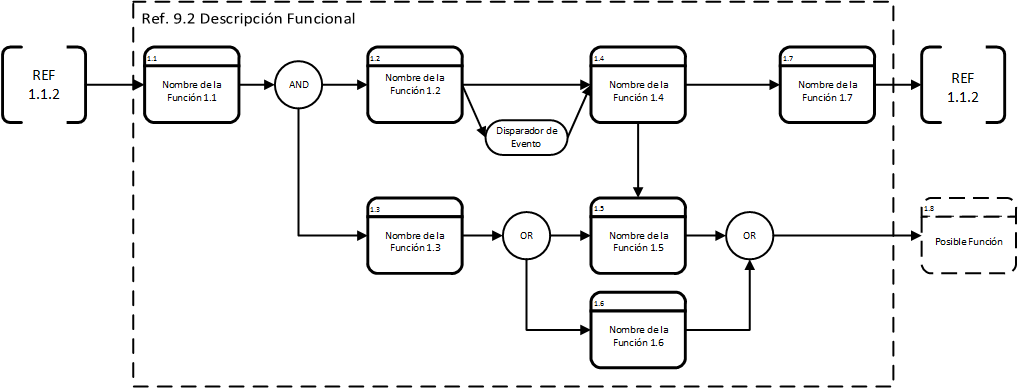
\includegraphics[scale=0.5]{marcoref/eFFBD}
	\caption{Diagrama eFFBD.}
	\label{img:diagramaeFFBD}
\end{figure}

En la imagen \ref{img:diagramaeFFBD} se puede observar que la primera funci\'on en ejecutarse es la funci\'on $1.1$. Al finalizar la funci\'on $1.1$, las funciones $1.2$ y $1.3$ comienzan a ejecutarse en paralelo. Al finalizar estos procesos, la funci\'on $1.4$ podr\'a ejecutarse en paralelo con la funci\'on $1.5$ o $1.6$, pero no con ambas a la vez. Una vez acabado este procedimiento, la funci\'on $1.7$ se ejecuta y as\'i acaba el proceso completo.\\

\noindent Como se ha mencionado, el diagrama eFFBD permite entender el comportamiento del sistema a lo largo del tiempo de ejecuci\'on (a diferencia del diagrama IDEF0 explicado en la secci\'on \ref{subsec:idef0}, que s\'olo muestra la relaci\'on que hay entre las funciones, m\'as no su ejecuci\'on a lo largo del tiempo).

		\subsection{Proceso de an\'alisis jer\'arquico} \label{subsec:ahp}
El proceso de an\'alisis jer\'arquico (\textit{Analytic Hierarchy Process}, AHP) es un m\'etodo de evaluaci\'on multicriterio desarrollado por Thomas L. Saaty.\\

\noindent El m\'etodo AHP tiene como fin el poder optimizar la toma de decisiones ante un problema complejo. Esta herramienta es aplicada a la toma de decisiones en la que existen varias opciones y se debe elegir la m\'as adecuada con base en los criterios considerados \cite{saaty_2008}. El m\'etodo de evaluaci\'on AHP contempla la experiencia del personal involucrado en la toma de la decisi\'on, junto con la informaci\'on cuantitativa del problema.\\

\noindent El m\'etodo AHP est\'a fundamentado en lo siguiente:

\begin{itemize}
	\item Toma de decisi\'on con base en los criterios planteados.
	\item Comparaciones por pares entre elementos con base en los criterios.
	\item Evaluaci\'on de los elementos mediante asignaciones de pesos.
	\item Priorizaci\'on de las alternativas de acuerdo a los pesos asignados.
\end{itemize}

%*************************************************************************************************************************************%	
	\section{Fundamentos del problema} \label{sec:basics}
		\subsection{CanSat} \label{subsec:cansat}
Un CanSat es una simulaci\'on de un sat\'elite real pero con el tama\~{n}o de una lata de refresco\footnote{Las dimensiones del CanSat dise\~{n}ado en este trabajo corresponden a las especificadas por la competencia \textit{Annual CanSat Competition} y que son, por requerimiento, mayores a las de una lata de refresco.}.\\

\noindent Los CanSats son peque\~{n}os dispositivos compuestos por diferentes elementos mec\'anicos y electr\'onicos cuyo prop\'osito es simular una misi\'on de un sat\'elite de gran escala. Estos dispositivos son elevados unos cuantos cientos de metros para despu\'es ser liberados. Los CanSats pueden tener alg\'un medio de reducci\'on de velocidad (paraca\'idas, serpentinas, h\'elices, escudo de calor, etc.) o descender en ca\'ida libre. Durante todo el tiempo de vuelo los CanSats com\'unmente env\'ian datos de variables atmosf\'ericas como presi\'on atmosf\'erica, temperatura y humedad. Estos dispositivos pueden variar en especificaciones de acuerdo a la misi\'on, sin embargo, presentan siempre similitudes en cuanto a las tareas b\'asicas de telemetr\'ia.\\

\noindent Los CanSats son usados mayormente con prop\'ositos educativos y proveen a los estudiantes involucrados en su dise\~{n}o de m\'ultiples responsabilidades, que van desde la concepci\'on de la misi\'on, hasta la integraci\'on de los elementos. Estos dispositivos pretenden integrar m\'ultiples \'areas del conocimiento y encaminarlas a la gesti\'on de un proyecto de tipo aeroespacial.

		\subsection{Fen\'omeno de autorrotaci\'on} \label{subsec:autorot}
Las aereonaves de ala rotativa son aquellas en la que la fuerza de sustentaci\'on se logra mediante el giro de alas o palas impulsadas por el aire y no por ning\'un tipo de motor. Las tres fuerzas principales que act\'uan sobre una pala del rotor son la fuerza de sustentaci\'on, $\overrightarrow{\text{dL}}$, la fuerza de arrastre, $\overrightarrow{\text{dD}}$, y la fuerza centr\'ifuga $\overrightarrow{\text{F}_\text{c}}$. La fuerza de sustentaci\'on es la fuerza hacia arriba causada por la interacci\'on entre el flujo de aire y el perfil aereodin\'amico. La fuerza de arrastre es quella que se opone al movimiento de la superficie de sustentaci\'on. La fuerza centr\'ifuga representa la tendencia de la pala del rotor a volar lejos del centro. Debido al movimiento circular, la velocidad del aire es mucho m\'as alta en la punta de la pala que en la base. La figura \ref{img:Helicoptero} muestra c\'omo act\'uan estas fuerzas en una aereonave de ala rotativa, en este caso, un helic\'optero.

\begin{figure}[H]
	\centering
		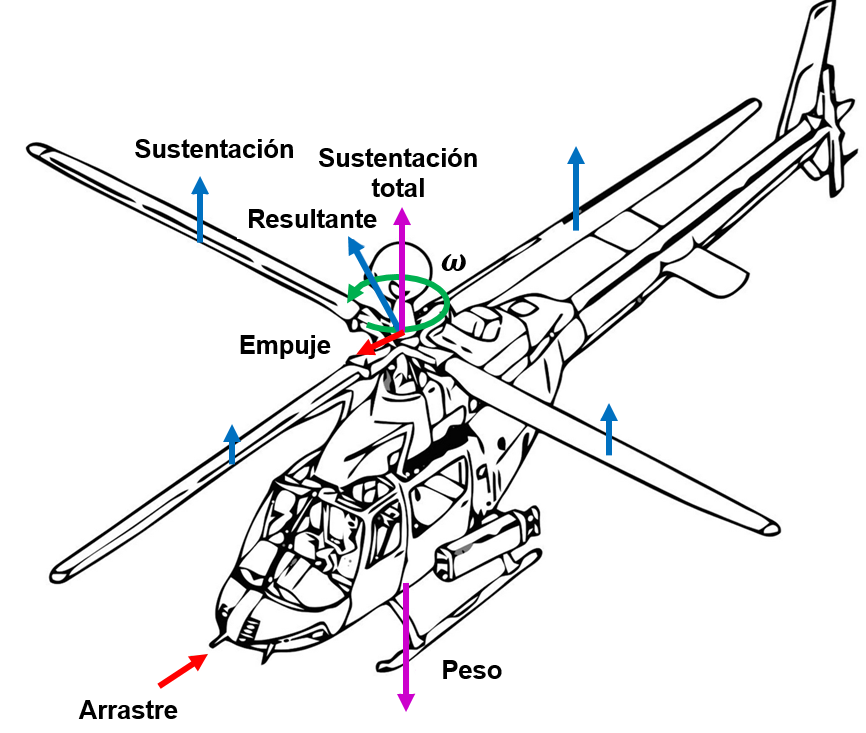
\includegraphics[scale=0.35]{imgmeca/Helicoptero.png}
	\caption{Fuerzas que act\'uan en el vuelo de una aereonave de ala rotativa.}
	\label{img:Helicoptero}
\end{figure}

\noindent La autorrotaci\'on  es un estado de vuelo que se presenta cuando el rotor principal de una aereonave de ala rotativa es movido por acci\'on del aire que va de abajo hacia arriba, y no precisamente por el motor o motores de la aereonave \cite{autorotation_2008}. En la autorrotaci\'on la corriente del aire entra desde la zona inferior del rotor y genera fuerzas aereodin\'amicas que lo mantienen en movimiento. Es el comportamiento habitual de los generadores e\'olicos, en los que el rotor extrae energ\'ia de la corriente de aire. Este fen\'omeno se muestra en la imagen \ref{img:Autorrotacion}.

\begin{figure}[H]
	\centering
		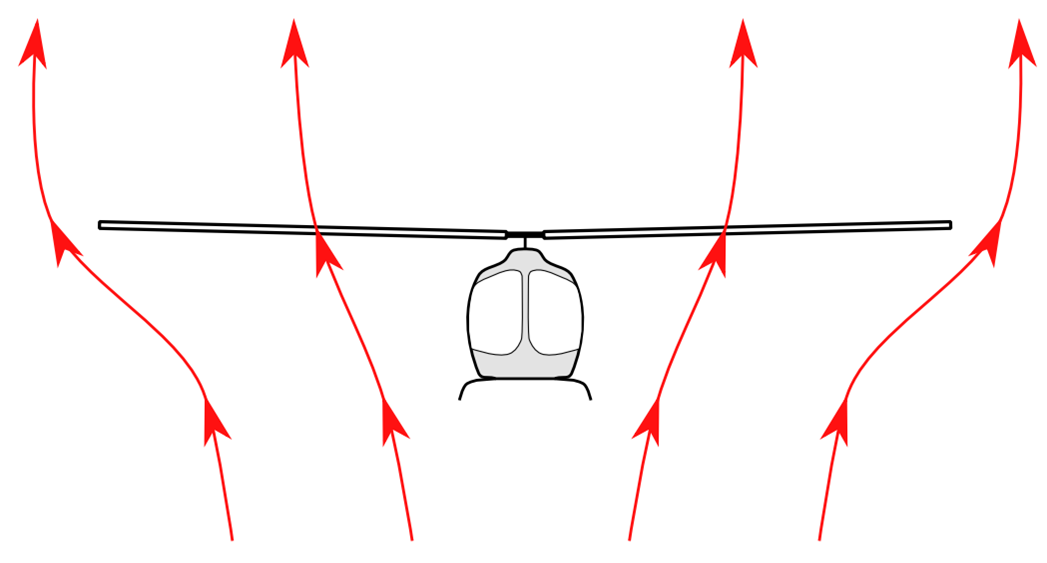
\includegraphics[scale=0.27]{imgmeca/Autorrotacion.png}
	\caption{Autorrotaci\'on. En rojo se muestran las l\'ineas de corriente con la direcci\'on de la velocidad de la corriente de aire.}
	\label{img:Autorrotacion}
\end{figure}


\noindent En este fen\'omeno la corriente de aire mantiene en movimiento a la aereonave de ala rotativa, ya que la sustentaci\'on es perpendicular a la corriente incidente y genera una fuerza que pone en movimiento las palas. Conforme vaya girando el rotor, el vector de fuerzas aereodin\'amicas de cada pala ir\'a girando hacia arriba, frenando la ca\'ida de la aereonave.\\

\noindent En relaci\'on a la geometr\'ia de las palas, los \'agulos de entrada de corriente son mayores en la zona de la ra\'iz de la pala, mientras que en  la punta son menores. Por lo tanto:

\begin{itemize}
\item Las zonas interiores de la pala presentan \'angulos de ataque grandes y la sustentaci\'on se orienta en la misma direcci\'on que la velocidad de rotaci\'on por lo que \'esta produce la potencia.
\item La zona de la punta de la pala presenta \'angulos de ataque peque\~{n}os y la sustentaci\'on se orienta en direcci\'on opuesta a la velocidad de rotaci\'on por lo que esta zona consume potencia.
\item En la condici\'on de autorrotaci\'on el par neto comunicado por esta confguraci\'on es nulo. La velocidad del rotor se ajustar\'a hasta alacanzar el equilibrio entre las fuerzas de inercia de rotaci\'on y las fuerzas aereodin\'amicas.
\end{itemize}
 
\noindent La figura \ref{img:Potencia} muestra las zonas productora y la zona consumidora de potencia durante la autorrotaci\'on.

\begin{figure}[H]
	\centering
	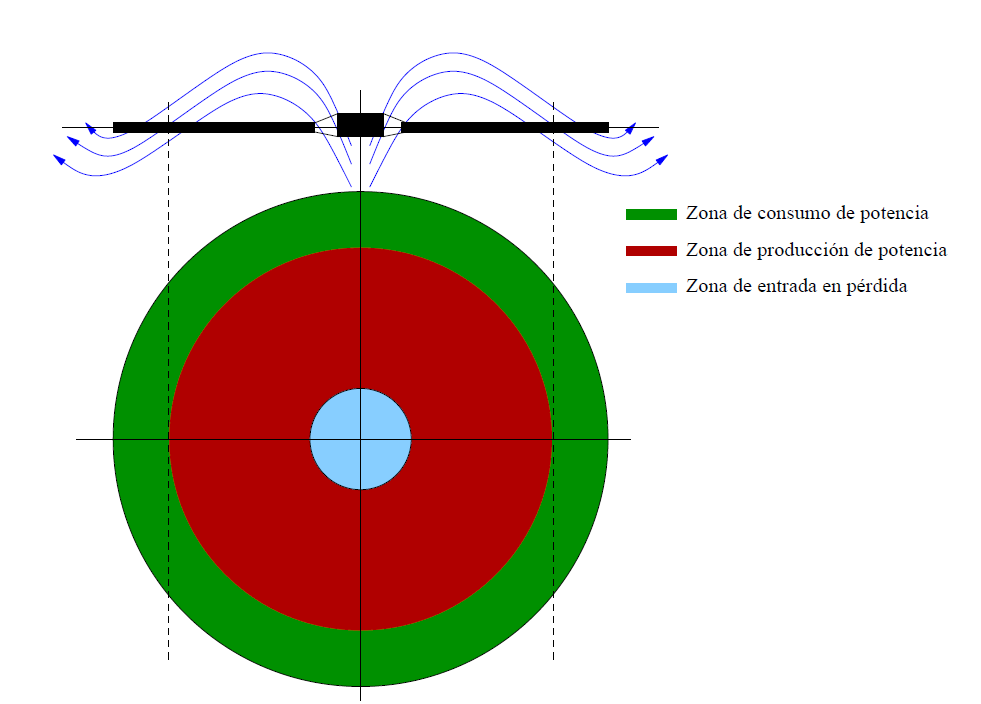
\includegraphics[scale=0.45]{imgmeca/Potencia.png}
	\caption{Zonas cosumidoras y productoras de potencia en el rotor durante el fen\'omeno de autorrotaci\'on.}
	\label{img:Potencia}
\end{figure}

\noindent Existe una zona en el rotor que ni consume ni genera potencia durante la autorrotaci\'on. En esta secci\'on las fuerzas tangenciales con nulas y s\'olo se produce el empuje. En la figura \ref{img:Secciones} la seccci\'on A corresponde con la caracter\'istica en autorrotaci\'on, la B como una secci\'on generadora de potencia y la C como una zona consumidora de potencia.

\begin{figure}[H]
	\centering
	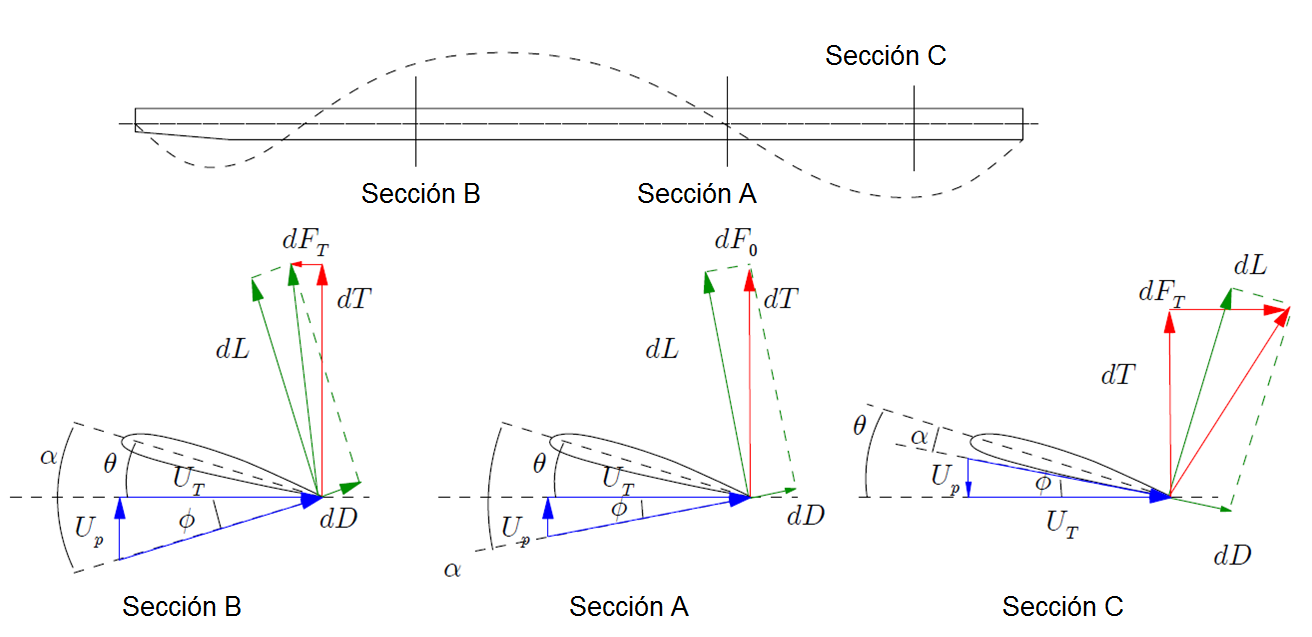
\includegraphics[scale=0.35]{imgmeca/Secciones.png}
	\caption{Secciones de h\'elice durante el fen\'omeno de autorrotaci\'on.}
	\label{img:Secciones}
\end{figure}

\noindent en donde $\text{dF}_{\text{T}}$ corresponde a la fuerza resultante entre la fuerza de arrastre y la fuerza de sustentaci\'on; $\text{U}_{p}$ y $\text{U}_{T}$ corresponden a los componenetes de la velocidad de viento perpendicular y tangencial, respectivamente; $\phi$ representa el \'angulo de entrada de corriente; $\theta$ es el \'angulo de paso y $\alpha$ es el \'angulo de ataque.
